\documentclass[a4]{report}
\usepackage{microtype}
\usepackage{xcolor}
\usepackage{minted}
\usepackage{hyperref}
\usepackage{fancyhdr}
\usepackage{graphicx}
\pagestyle{fancy}


\newcommand{\hrefinternal}[2]{#2}%
\fancyhf{}                              % delete the current header and footer
\fancyhead[LO]{\parbox[t]{0.9\textwidth}{\textbf{\rightmark}}} %<--- use [t] for parbox.
\fancyhead[RO]{\parbox[t]{0.02\textwidth}{\textbf{\thepage}}} %<--- better use [t]  here also for parbox to ensure that alignmen


\begin{document}
\title{Adaptive Sampling Kit v\input{../VERSION} Documentation}

\maketitle
\tableofcontents

\break
 \begin{center}

   \textbf{Adaptive Sampling Kit v\input{../VERSION} Documentation} 

 \bigskip
     \texttt{Pablo de Oliveira Castro, ECR/UVSQ}
 \bigskip
 
\end{center}

Adaptive Sampling Kit (ASK) is a toolkit for sampling big experimental spaces. It features multiple active learning algorithms to prioritize the exploration of the interesting parts of the experimental space.

\paragraph{}
\noindent Copyright \copyright2011-2012 Universit\'e de Versailles St-Quentin-en-Yvelines
\paragraph{}
\noindent Permission is granted to copy, distribute and/or modify this document
under the terms of the GNU Free Documentation License, Version 1.3
or any later version published by the Free Software Foundation;
with no Invariant Sections, no Front-Cover Texts, and no Back-Cover Texts.
A copy of the license is included in the section entitled "GNU
Free Documentation License".
\paragraph{}
The Adaptive Sampling Kit (ASK) is released under the GNU 
General Public License, version 2. Please refer to the file LICENSE that 
accompanies your copy of ASK. 


\section*{Acknowledgments}
This work has been done in the Exascale Computing Research lab, thanks to the support of CEA, GENCI, Intel and UVSQ.

\section*{Contact}
For any question regarding ASK, please write at \href{mailto:ask-team@exascale-computing.eu}{ask-team@exascale-computing.eu}

\section*{Contributors}
\begin{itemize}
	\item Pablo de Oliveira Castro, wrote ASK and its documentation
	\item Eric Petit contributed many ideas during ASK development and evaluated ASK on two performance case-studies
	\item E. Beyler, J.C. Beyler, and B. Krammer, reviewed extensively this documentation 
	\item The members of the Exascale Computing research lab, which provided useful code reviews
\end{itemize}

\chapter{General Information}
\section{Introduction}

ASK stands for Adaptive Sampling Kit. Its main goal is accelerating long experiments. Two kinds of variables define an experiment: a response and a set of factors. The response is characterized on the factors' Cartesian product.

When the space is small, the response can be measured for every point in the space. When the space is large, doing an exhaustive measurement is either not possible in terms of execution time or simply not practical. ASK tries to find good approximations of the response by sampling only a small fraction of the space.

\section{How Does It Work?}

ASK tries to efficiently sample the space by using \emph{active learning}, also called \emph{adaptive sampling}, approaches.
These approaches can usually be broken into three steps:
\begin{itemize}
	\item First, they sample a few points in the space and evaluate the response on the space by building a model.
\end{itemize}

\begin{itemize}
	\item Second, they identify the regions of the space where the model is \emph{imprecise}. The exact definition of \emph{imprecise} depends on each particular approach.
\end{itemize}

\begin{itemize}
	\item Third, they sample new points by prioritizing the exploration of the \emph{imprecise} regions. In other terms, they concentrate on the regions where interesting things happen.
\end{itemize}

\section{ASK Organization}

ASK is organized as a toolkit, composed of different modules with well-defined roles:

\begin{itemize}
	\item Bootstrap modules: select an initial batch of points to measure
\end{itemize}

\begin{itemize}
	\item Sampler modules: use adaptive sampling techniques that find interesting points to sample
\end{itemize}

\begin{itemize}
	\item Model modules: model the full space response based on a set of sampled points
\end{itemize}

\begin{itemize}
	\item Source modules: gather data by running experiments or by reading data from a database
\end{itemize}

\begin{itemize}
	\item Report modules: report statistics and plots to the user
\end{itemize}

A driver, called \texttt{ask}, orchestrates the communication and set-up of all these modules.


\chapter{Installation and First Use}
\section{Introduction}

The following chapter presents how to download and configure ASK on the user's workstation.

\section{Download}

Download ASK through the Git version control system:

\begin{minted}{bash}
$ git clone https://code.google.com/p/adaptive-sampling-kit/
\end{minted}

The previous command retrieves the current stable version of ASK. To switch to the development version type:

\begin{minted}{bash}
$ cd ask
$ git checkout develop
\end{minted}

\section{Configuration}

Before using ASK, make sure all its dependencies are satisfied:

\begin{itemize}
	\item Python: at least version 2.6
\end{itemize}

\begin{itemize}
	\item R
\end{itemize}

\begin{itemize}
	\item Libraries: python-numpy, python-scipy and python-argparse
\end{itemize}

\begin{itemize}
	\item Optionally, nosetests, which is only needed to \hrefinternal{http:///wiki/Application\_Characterization:\_ASK:\_Chapter\_6:\_Support\#Running\_the\_Test\_Suite}{run the regression test suite}
\end{itemize}

In a Debian or Ubuntu system, use:

\begin{minted}{bash}
$ sudo apt-get install python2.6 r-base python-numpy python-scipy \
       python-argparse python-nose
\end{minted}

Ensure that R\_LIBS contains a writable directory. For example, add the following line to your \texttt{.bashrc}, or equivalent, file:
\begin{minted}{bash}
export R_LIBS=$HOME/.R-libs:$R_LIBS
\end{minted}

and create the directory with:
\begin{minted}{bash}
$ mkdir $HOME/.R-libs/
\end{minted}

Once the dependencies are installed and R\_LIBS configured, enter ASK's directory and execute the \texttt{configure} script.

\begin{minted}{bash}
$./configure
Checking if R is installed
Checking if python is installed
All the dependencies are satisfied.
Building uniform sampling dynamic library (only needed for amart sampler module)
\end{minted}

The configure script makes sure all previous dependencies are properly installed.
It also retrieves a set of R modules from \href{http://cran.r-project.org/}{rcran}.
Therefore, before running this script, make sure the computer is connected to the internet.

ASK installation is self-contained: it does not install system-wide files. The \texttt{ask} binary can be run directly, or added to 
the PATH environment variable, eg. in bash:
\begin{minted}{bash}
cd ask/
export PATH=$PWD:$PATH
\end{minted}

The ASK directory contains the following subdirectories:

\begin{itemize}
	\item \texttt{common/}, contains common libraries
\end{itemize}

\begin{itemize}
	\item \texttt{examples/}, contains runable examples of ASK's usage
\end{itemize}

\begin{itemize}
	\item \texttt{tests/}, contains the \hrefinternal{http:///wiki/Application\_Characterization:\_ASK:\_Chapter\_6:\_Support\#Running\_the\_Test\_Suite}{test regression suite}
\end{itemize}

\begin{itemize}
	\item \texttt{bootstrap/}, contains the standard \hrefinternal{http:///wiki/Application\_Characterization:\_ASK:\_Chapter\_4:\_Standard\_Modules\#Bootstrap\_Modules}{Bootstrap modules}
\end{itemize}

\begin{itemize}
	\item \texttt{control/}, contains the standard \hrefinternal{http:///wiki/Application\_Characterization:\_ASK:\_Chapter\_4:\_Standard\_Modules\#Control\_Modules}{Control modules}
\end{itemize}

\begin{itemize}
	\item \texttt{model/}, contains the standard \hrefinternal{http:///wiki/Application\_Characterization:\_ASK:\_Chapter\_4:\_Standard\_Modules\#Model\_Modules}{Model modules}
\end{itemize}

\begin{itemize}
	\item \texttt{reporter/}, contains the standard \hrefinternal{http:///wiki/Application\_Characterization:\_ASK:\_Chapter\_4:\_Standard\_Modules\#Reporter\_Modules}{Reporter modules}
\end{itemize}

\begin{itemize}
	\item \texttt{sampler/}, contains the standard \hrefinternal{http:///wiki/Application\_Characterization:\_ASK:\_Chapter\_4:\_Standard\_Modules\#Sampler\_Modules}{Sampler modules}
\end{itemize}

\begin{itemize}
	\item \texttt{source/}, contains the standard \hrefinternal{http:///wiki/Application\_Characterization:\_ASK:\_Chapter\_4:\_Standard\_Modules\#Source\_Modules}{Source modules}
\end{itemize}

\begin{itemize}
	\item \texttt{utils/}, contains two scripts handling time series, described in \hrefinternal{http:///wiki/Application\_Characterization:\_ASK:\_Chapter\_3:\_Experiment\_Setup\#Analyzing\_the\_experiment}{Chapter 3}
\end{itemize}

\section{First Use}

Go into ASK's directory and type \texttt{ask -h} to get a brief summary of the command-line options.
\hrefinternal{http:///wiki/Application\_Characterization:\_ASK:\_Chapter\_3:\_Experiment\_Setup\#ASK\_invocation}{Chapter 3} explains in detail ASK's invocation.

Now, consider the \texttt{simple} experiment from the \texttt{examples} directory.

\begin{minted}{bash}
$ cd ask/; export PATH=$PWD:$PATH
$ cd examples/simple
$ ls 
gauss2D.data simple.conf
\end{minted}

Observe there are two files:

\begin{itemize}
	\item \texttt{Gauss2D.data} contains some measures:
\end{itemize}

\begin{minted}{rconsole}
-200 -200 -0.000670925255805024
-199 -200 -0.000694745225748637
-198 -200 -0.000719248849372865
-197 -200 -0.00074444881633483
-196 -200 -0.00077035776068282
-195 -200 -0.0007969882457312
-194 -200 -0.000824352748414127
-193 -200 -0.00085246364311948
-192 -200 -0.000881333185005384
-191 -200 -0.000910973492802606
...
\end{minted}

The last column represents the response; the first two columns are factors.

The above file contains an exhaustive measure of a design space inspired by an example from the article, \emph{tgp: An R package for Bayesian nonstationary, semiparametric nonlinear regression and design by treed gaussian process models. }, R. B. Gramacy, Journal of Statistical Software 2007: 

$$
f(x_1,x_2) = \frac{x_1}{100}.e^{-(\frac{x_1}{100})^2-(\frac{x_2}{100})^2} \textrm{ on } [-200:600] \times [-200:600]
$$

The design space has two factors, named x1 and x2 in the formula, and the response f(x1,x2).

\begin{itemize}
	\item \texttt{Simple.conf} contains the configuration of the experiment
\end{itemize}

The configuration file's first section, named factors, describes the factors of the experiment:

\begin{minted}{js}
"factors": [
  {"name": "x",
   "type": "integer",
   "range": {"min": -200, "max": 600}
  },
  {"name": "y",
   "type": "integer",
   "range": {"min": -200, "max": 600}
  }
]
\end{minted}

In the experiment, there are two factors called \textbf{x} and \textbf{y}, both of type \textbf{integer} and varying between -200 and 600, bounds included.

The second section, Modules, configures the ask modules involved in this experiment. The bootstrap module samples five hundred points random points, a general boosting machine (gbm) model is built and the 2D reporter plots the result. For a full discussion of module parameters please refer to \hrefinternal{http:///wiki/Application_Characterization:_ASK:_Chapter_3:_General_Usage}{Chapter 3}. 

To run the experiments, type:

\begin{minted}{bash}
$ ask simple.conf
Logging to default.log
Experiments finished normally
\end{minted}

The ask driver runs approximately for one minute and reports that the experiment finished without errors. While it is running, the \texttt{default.log} file tracks the driver's progress, the default.log file is created by default in the directory where ASK is invoked. ASK saves all the results into the default output directory \texttt{output/}:

\begin{minted}{bash}
$ ls output/
labelled00000.data  labelled.data  model00000.data  plot00000.png  
prediction00000.data
\end{minted}

Open the \texttt{plot00000.png} file in an image viewer, observe it shows two level plots:

\begin{itemize}
	\item The top one, shows the absolute error between the response model and the true response: white is better
\end{itemize}

\begin{itemize}
	\item The bottom one, shows the response model built using five hundred samples
\end{itemize}

\begin{itemize}
	\item The samples themselves are marked by the tiny circles
\end{itemize}

\begin{center}
  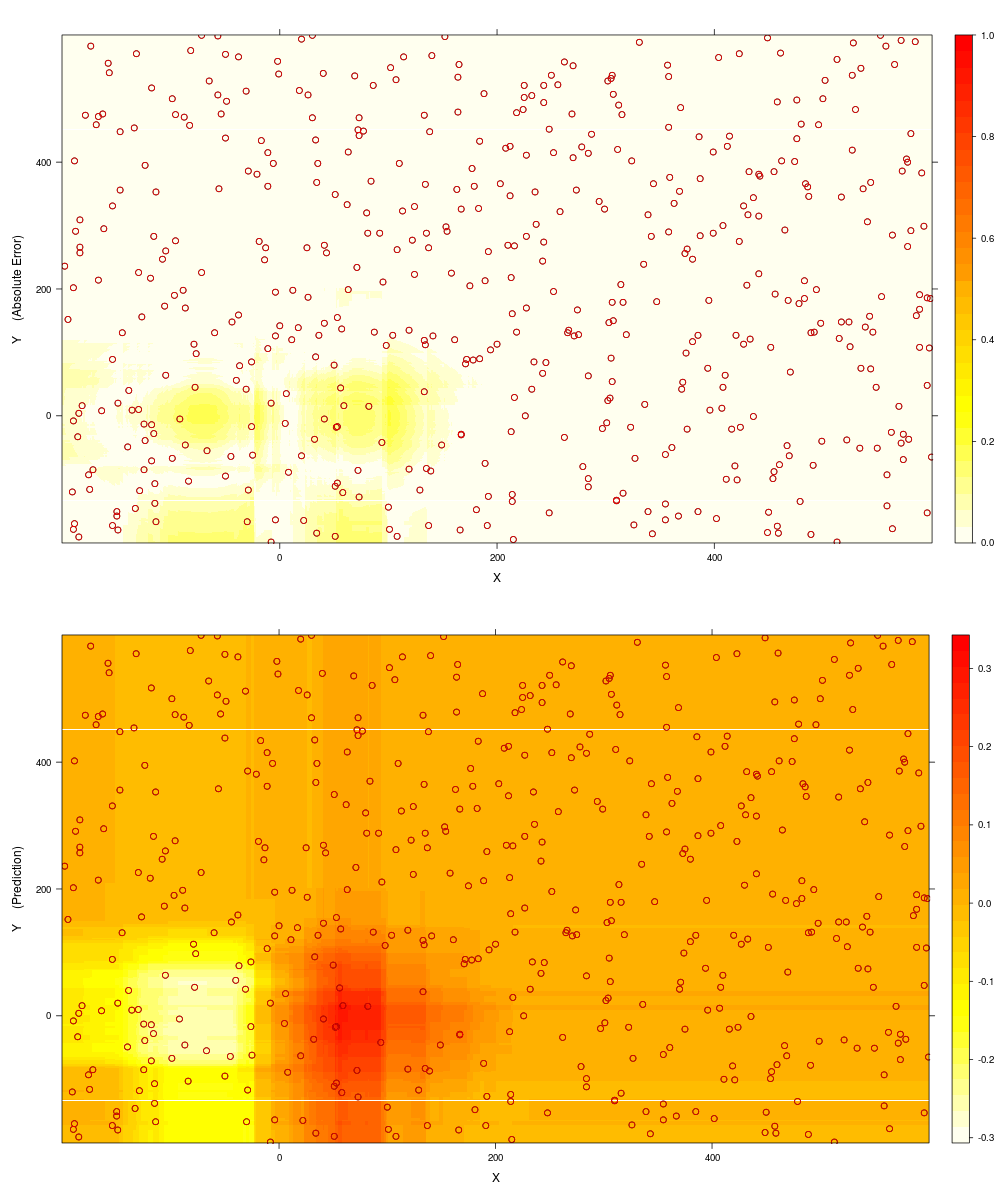
\includegraphics[width=\textwidth]{figures/ASK-first-plot.png}
\end{center}





\chapter{Experiment Setup}
\section{ASK Configuration}

\subsection{Introduction: ASK Module Pipeline}

ASK's flexibility and extensibility come from its modular architecture. When running an experiment, ASK follows the pipeline below,


\begin{center}
  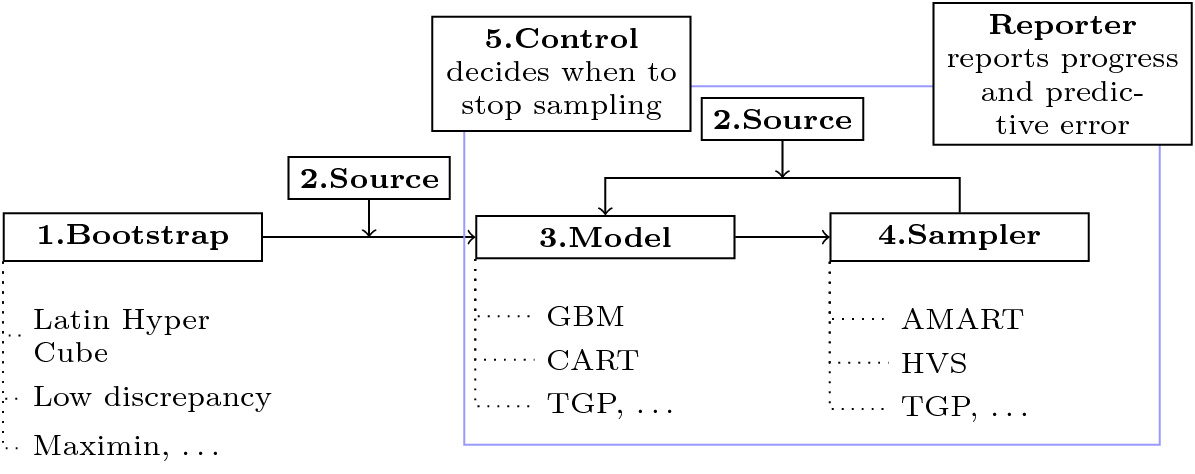
\includegraphics[width=\textwidth]{figures/ASK-modules-pipeline.png}
\end{center}


First, the \textbf{Bootstrap} module selects a set of initial points to measure. The initial selection is passed to the \textbf{Source} module which runs an experiment for each point and returns the measured response. A \textbf{Model} module fits the first set of measures to a surrogate model, producing a first prediction of the response on the full design space. Since the prediction is still very rough, the \textbf{Sampler} modules chooses additional points to measure that will improve the model accuracy. The sampler selected points are measured with the \textbf{Source} module and fitted again in the model.
The \textbf{Control} module is in charge of stopping the process after a fixed number of iteration or when a quality threshold is reached. Finally, the \textbf{Reporter} module produces informative statistics for the user during the experiment.

ASK offers different implementations for each module. It allows building customized experimental pipelines. If one feature is missing, users can write their own module implementing it.

\subsection{ASK invocation}

The coordination between the modules is entirely handled by ASK. 
Before running an experiment, the user must prepare a configuration file describing the experiment's parameters and the selected modules.
Once the configuration file is ready, the user should type,

\begin{minted}{bash}
$ ask <configuration_file>
\end{minted}

Any fatal error stops the execution and is immediately reported to the user. Warnings are logged to a log file. By default the log file name is \texttt{default.log}. All the samples measured, models built and reports produced are saved inside an output directory, which is by default called \texttt{output/}. The configuration file allows changing both the log file name and the output directory names.

The following command line flags alter the default behavior:

\begin{itemize}
	\item \texttt{-h} or \texttt{--help}, returns a short message describing the available flags and their usage.
	\item \texttt{--force\_overwrite}, to prevent accidental loss of experiment data, ASK refuses to run if the output directory already exist in the current path. If this option is used ASK will overwrite the previous output directory with the new experiments.
	\item \texttt{--skip\_reporter}, this flag runs an ASK experiment by skipping calls to the Reporter module. This is useful for long runs on which the user will not supervise the execution and wants to avoid the overhead of generating reports.
	\item \texttt{--skip\_model}, this flag runs an ASK experiment by skipping calls to the Model module. Beware; if the Reporter or Sampler module you use require a surrogate model, using this flag will raise an error at execution.
	\item \texttt{--replay\_only}, this flag requires that a previously created output directory exists. It replays a previous ASK experiment bypassing calls to the source, sampler, and bootstrap modules. This enables reusing old measures with a new reporter or model module. A common scenario for this flag is doing experiments on a remote machine, where calling the reporter module is unnecessary, retrieving the data on the experimenter's local computer, and replaying the experiments with the reporter module enabled to analyze the results.
\end{itemize}

\begin{minted}{bash}
$ ./ask -h
usage: ask [-h] [--force_overwrite] [--replay_only] [--skip_model]
           [--skip_reporter]
           configuration

Helps choosing sampling points during experiments.

positional arguments:
  configuration      the experiment configuration file

optional arguments:
  -h, --help         show this help message and exit
  --force_overwrite  If a previous output directory is found its contents will
                     be overwritten
  --replay_only      (Must be run over a full previous ask run). Skip
                     bootstrap and sampler modules, but runs previous labels
                     through the model and reporter. This option is useful if
                     one wants to run sampling and analyze results separately.
  --skip_model       Skip model module. (WARNING: if the chosen control module
                     relies on the output of the model module, this option
                     fails.)
  --skip_reporter    Skip reporter module. (WARNING: if the chosen control
                     module relies on the output of the reporter module, this
                     option fails.)
\end{minted}

\subsection{ASK Configuration File}

This section describes the ASK configuration file format. The ASK configuration file follows the \href{http://www.json.org/}{JavaScript Object Notation (JSON)} format. The simple example of \hrefinternal{http:///wiki/Application_Characterization:_ASK:_Chapter_2:_Installation_and_First_Use}{Chapter 2} is presented below.

\begin{minted}{js}
{
  "factors": [
    {"name": "x",
     "type": "integer",
     "range": {"min": -200, "max": 600}
    },
    {"name": "y",
     "type": "integer",
     "range": {"min": -200, "max": 600}
    }
  ],
  "modules": {
    "bootstrap": {
      "executable": "bootstrap/random",
      "params": {        
        "n": 500
      }
    },
    "source": {
      "executable": "source/file",
      "params": {
        "data_file": "gauss2D.data"
      }
    },
    "model": {
      "executable": "model/gbm_build",
      "predictor": "model/gbm_predict",
      "params": {"ntrees":100, "interactiondepth": 5, "shrinkage":0.1}
    },
    "sampler": {
      "executable": "sampler/hierarchical",
      "params": {
        "cp":0.01,
        "n":50,
        "ponderate_by_size":false
      }
    },
    "control": {
      "executable": "control/points",
      "params": {
        "n": 500
      }
    },
    "reporter": {
      "executable": "reporter/generic/report",
      "params": {
        "test_set": "gauss2D.data",
        "max_error_scale": 1,
        "timeseries": "simple_timeseries.out",
        "script": "reporter/generic/2D.R"
      }
    }
  },
  "log": {
    "logfile": "default.log",
    "level": "DEBUG"
  },
  "output_directory": "output/"
}
\end{minted}

There are four outer level sections:
\begin{itemize}
	\item \texttt{output\_directory} specifies the name of the output directory.
	\item \texttt{log} specifies the name of the log file and the log level. There are five log levels: DEBUG, INFO, WARNING, ERROR, and CRITICAL. The higher the log level the less messages are logged.
	\item \texttt{factors} section configures the experiment's factors.
	\item \texttt{modules} section configures the modules.
\end{itemize}

Factors and most modules sections are mandatory. Nevertheless, some sections are optional: output\_directory, log, modules.model, and modules.reporter. Sane default values replace optional missing sections, the default values can be changed by editing the file \texttt{ask/default.conf}. 

\subsubsection{Factors Section}

The factors section describes each of the factors, sometimes called independent variables, of your experiment.
Each factor can take different values. The response, sometimes called dependent variable, will be measured and 
predicted for different combinations of the factors values.

Below is a factors section demonstrating all the different types of factors available in ASK.

\begin{minted}{js}
"factors": [
  {"name": "number_of_threads",
  "type": "integer",
  "range": {"min": 1, "max": 32}
  },
  {"name": "seed",
  "type": "float",
  "range": {"min": -10.3, "max": 3.1415}
  },
  {"name": "cache_level",
  "type": "categorical",
  "values": ["L1", "L2", "L3"]
  },
],
\end{minted}

The factors section is an array of factors. Each factor is an object with three attributes:
\begin{itemize}
	\item \texttt{name}, contains a unique string identifying the factor.
	\item \texttt{type}, describes the type of factor. There are three valid types:
	\begin{itemize}
		\item \texttt{integer}, represent an integer factor bounded by a minimum and maximum value.
		\item \texttt{float}, represents a real factor bounded by a minimum and maximum value.
		\item \texttt{categorical}, represents a discrete factor that can take a finite number of categorical values. No order is assumed among the values.
	\end{itemize}
	\item The third attribute determines the admissible values for the factor. The name of the third attribute depends on the type of factor. For \texttt{integer} or \texttt{float} types the third attribute is \texttt{range}; for \texttt{categorical} type, the third attribute is \texttt{values}.
	\begin{itemize}
		\item \texttt{range}, is an object with two attributes \texttt{min} and \texttt{max} giving the inclusive lower and upper bounds of the factor.
		\item \texttt{values}, is an array of strings. Each string corresponds to a possible value of the categorical factor.
	\end{itemize}
\end{itemize}

\subsubsection{Modules Section}

The module section selects for each module one specific implementation and if needed configures the module parameters.

\begin{minted}{js}
"modules": {
  "bootstrap": {
    "executable": "bootstrap/random",
    "params": {
      "n": 500
    }
  },
  "control": {
    "executable": "control/points",
    "params": {
      "n": 500
    }
  },
  "reporter": {
    "executable": "reporter/generic/report",
    "params": {
      "test_set": "gauss2D.data",
      "max_error_scale": 1,
      "timeseries": "simple_timeseries.out",
      "script": "reporter/generic/2D.R"
    }
  },
  "source": {
    "executable": "source/file",
    "params": {
      "data_file": "gauss2D.data"
    }
  },
  "sampler": {
    "executable": "sampler/hierarchical",
    "params": {
      "cp":0.01,
      "n":50,
      "ponderate_by_size":false
    }
  },
  "model": {
    "executable": "model/gbm_build",
    "predictor": "model/gbm_predict",
    "params": {"ntrees":100, "interactiondepth": 5, "shrinkage":0.1}
  }
},
\end{minted}

The order of the modules instantiations is not important.
Each module subsubsection contains two parameters:
\begin{itemize}
	\item \texttt{executable}, which contains the path of the module's chosen instance. Each instance is an executable file. The path can be absolute or relative to the current directory or to ASK's root directory; path resolution proceeds in this exact order.
	\item \texttt{params}, contains a list of module specific parameters. The format of \texttt{params} is module dependent, \hrefinternal{http:///wiki/Application_Characterization:_ASK:_Chapter_4:_Standard_Modules}{Chapter 4} describes the parameters expected by each module.
\end{itemize}

Model modules are an exception. Indeed, a model module responsibilities are two-fold:
\begin{itemize}
	\item building models from sampled data
	\item predicting the response on new data
\end{itemize}

The model subsubsection expects the executable for building a model in the \texttt{executable} field. It contains an additional parameter, 
\texttt{predictor} that gives the path of the module's predictor path.

\subsection{Data Exchange Format}

This section describes the format used by ASK modules to exchange points and their response.
The format is in space separated values format.
Let \textbf{n} be the number of factors declared in the \hrefinternal{http:///wiki/Application_Characterization:_ASK:_Chapter_3:_Experiment_Setup\#ASK_Configuration_File}{Factors section} of the configuration file.

Each line of the file represents a point in the space. The first \textbf{n} columns represent the factor values in the order of the \hrefinternal{http:///wiki/Application_Characterization:_ASK:_Chapter_3:_Experiment_Setup\#ASK_Configuration_File}{Factors section}. If a \textbf{n+1} column is added, it represents the response measured for this factor combination.

The file below contains four points, the first five columns are the factors coordinates, and the sixth column contains the response:

\begin{minted}{bash}
1 64 64 0 4 109.728
12 314 1064 4 0 9.14235
1 314 1064 4 1 115.078
4 564 64 0 0 9.01366
\end{minted}

\section{Setting Up an Experiment}

This section explains systematically how to setup an ASK experiment using the 2D synthetic design space that was used in \hrefinternal{http:///wiki/Application\_Characterization:\_ASK:\_Chapter\_2:\_Installation\_and\_First\_Use\#First\_Use}{Chapter 2}:


$$
f(x_1,x_2) = \frac{x_1}{100}.e^{-(\frac{x_1}{100})^2-(\frac{x_2}{100})^2} \textrm{ on } [-200:600] \times [-200:600]
$$

The design space is inspired by an example from the article, \emph{tgp: An R package for Bayesian nonstationary, semiparametric nonlinear regression and design by treed gaussian process models}, R.B. Gramacy, Journal of Statistical Software 2007. 
The design space has two factors x1 and x2 and the response plotted below.

\begin{center}
  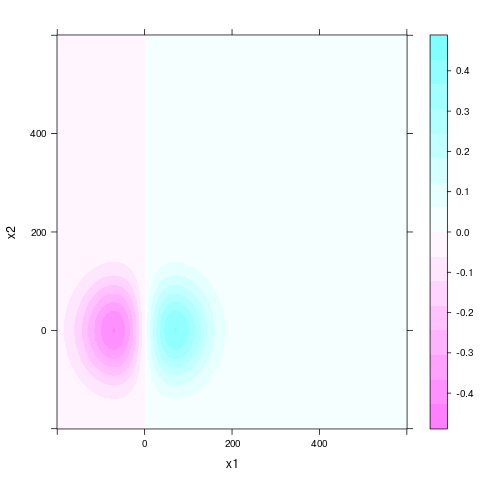
\includegraphics[width=\textwidth]{figures/ASK-gauss2D-ideal.png}
\end{center}



The configuration and set-up described below is available in the directory \texttt{ask/examples/gauss2D}.

\subsection{Writing a Source Module}

The first step is defining a source module to measure the response on any point of the space.
In the example, the module simply computes the response of the function f over the input points.
Below is a simple R implementation for the source module:

\begin{minted}{r}
#!/usr/bin/env Rscript
# A simple source module
# Parse the module arguments
args <- commandArgs(trailingOnly = T)
if (length(args) != 3) {
    stop("Usage: source <configuration.conf> <requested_file> <output_file>")
}

# Read the requested points
requested = read.table(args[2])

# Define the function to study
# (A real experiment would here call some measurement process)
myf <- function (x1,x2) {
  x1 = x1/100
  x2 = x2/100
  return (x1 * exp(-x1*x1 - x2*x2))
}

# Compute f over all the requested points
requested$response = myf(requested$V1, requested$V2)

# Write results
write.table(requested, args[3], sep=" ", quote=F, col.names=F, row.names=F)
\end{minted}

All \hrefinternal{http:///wiki/Application_Characterization:_ASK:_Chapter_5:_Writing_Modules\#Source_Modules}{source modules} take three arguments:
\begin{enumerate}
	\item The path of the experiment \hrefinternal{http:///wiki/\#ASK_Configuration_File}{configuration file}.
	\item The path of the requested points file. This file contains the list of space points to be measured, in \hrefinternal{http:///wiki/\#Data_Exchange_Format}{ASK's data exchange format}.
	\item The path of the output file.
\end{enumerate}

The above script conforms to this interface: first, it parses the three arguments. Then, it reads the list of points to measure. Conveniently, the data exchange format used by ASK can be read from R with the \texttt{read.table()} function. For each combination of factors \texttt{(x1,x2)}, the response is computed. Finally, the script writes each combination and its response to the output file.
The above source module is straightforward and does not need additional configuration; therefore, it ignores the configuration file parameter.

Checking that the above implementation works is simple. Prepare a requested file with a few points, for instance:

\begin{minted}{bash}
<file: some.data>
10 10 
50 -15.3 
200 -30 
\end{minted}

Prepare an empty configuration file, for now.
Then call the source module on this file:

\begin{minted}{bash}
$./source.R empty.conf some.data out.data
$cat out.data
10 10 0.0980198673306755
50 -15.3 0.3803907821641490
200 -30 0.0334784671171613
\end{minted}

As expected, the source module computes the response for each factor.
The source module is the interface between ASK and the user's experimental setup. The next section explains how to configure the rest of the experimental pipeline.

\subsection{Configuring the Factors}

To configure the experiment, write a \hrefinternal{http:///wiki/Application_Characterization:_ASK:_Chapter_3:_Experiment_Setup\#ASK_Configuration_File}{configuration file}.
Start with the \hrefinternal{http:///wiki/Application_Characterization:_ASK:_Chapter_3:_Experiment_Setup\#Factors_section}{Factors section} that describes the type and domain of the factors. The function f is defined on two float factors ranging from -200 to 600:

\begin{minted}{js}
"factors": [
  {"name": "x1",
   "type": "float",
   "range": {"min": -200, "max": 600}
  },
  {"name": "x2",
   "type": "float",
   "range": {"min": -200, "max": 600}
  }
],
\end{minted}

\subsection{Choosing and Configuring the Sampling Pipeline}

The next step is choosing and configuring the modules for the experiment.
One module must be chosen for each step of the \hrefinternal{http:///wiki/Application_Characterization:_ASK:_Chapter_3:_Experiment_Setup\#Introduction:_ASK_module_pipeline}{experimental pipeline}.

\subsubsection{Source Module}

First add the \hrefinternal{http:///wiki/\#Writing_a_Source_Module}{source module} that measures f. Remember, it is a simple R executable, called \texttt{source.R}.
\begin{minted}{js}
"modules": {
  "source": {
    "executable": "./source.R",
    "params": {}    
  }
}
\end{minted}

The script does not expect any configuration parameters so \texttt{"params"} is left empty.
Remember to set the executable bit of source.R before running the experiment.

\subsubsection{Bootstrap Module}

The bootstrap module selects the first batch of sampled points. ASK offers different standard bootstrap modules available in the \texttt{ask/bootstrap} directory and described in \hrefinternal{http:///wiki/Application_Characterization:_ASK:_Chapter_4:_Standard_Modules}{Chapter
4: Standard Modules}.

The example uses the \texttt{bootstrap/random} module that selects random factor combinations.

\begin{minted}{js}
"bootstrap":  {
  "executable": "bootstrap/random",
  "params": {"n": 50}
}
\end{minted}

The parameter \texttt{"n"} specifies that exactly 50 combinations should be sampled during bootstrap.

\subsubsection{Model Module}

The model module predicts the response in locations not yet sampled.
The example uses the \href{http://cran.r-project.org/web/packages/gbm/}{Generalized Boosted Model} with its default parameters.

\begin{minted}{js}
"model":  {
  "executable": "modules/gbm_build",
  "predictor": "model/gbm_predict",
  "params": {}
}
\end{minted}

When no parameters are specified, default values are provided.
GBM works by combining multiple tree predictors, the default number of trees is 3000.
To change this value to 1000, one would simply use the line:

\begin{minted}{js}
"params": {"ntrees":1000}
\end{minted}

\hrefinternal{http:///wiki/Application_Characterization:_ASK:_Chapter_4:_Standard_Modules}{Chapter 4: Standard Modules} describes the full set of available configuration.

\subsubsection{Sampler Module}

The sampler module samples additional points for every iteration of the experimental pipeline.
The examples uses the Hierarchical Variance Sampler included in ASK and samples 50 new points per iteration.

\begin{minted}{js}
"sampler": {
  "executable": "sampler/hierarchical",
  "params": {"n": 50}
}
\end{minted}

\subsubsection{Control Module}

The control module chooses when to end the experiment. The example uses the \texttt{points} control, which stops after a given number of points in sampled.

\begin{minted}{js}
"control": {
  "executable": "control/points",
  "params": {"n": 500}
}
\end{minted}

Here the experiment will stop after sampling 500 points, which amounts to one bootstrap sampling and nine Hierarchical Variance samplings.

\subsubsection{Report Module}

The report module produces detailed statistics about the sampling.
In this case, the generic reporter is used:

\begin{minted}{js}
"reporter": {
  "executable": "reporter/generic/report",
  "params": {
    "script": "reporter/generic/2D.R",
    "test_set": "test.data",
    "timeseries" : "timeseries.out"
  }
}
\end{minted}

The \texttt{script} parameter requires a script to plot the response prediction. ASK includes default scripts to handle 1D and 2D dimensions.
For higher dimensions, users must provide their own script.

The \texttt{test\_set} parameter is the path of a file containing a set of measures to use as a test set in \hrefinternal{http:///wiki/\#Data_Exchange_Format}{ASK's data exchange format}.

Finally, \texttt{timeseries} parameter is the path of an output file. The generic reporter module produces in this file the time series of the model accuracy. Plotting this time series is interesting to evaluate if the model converges.

\subsection{Running the Experiment}

To run the experiment type:

\begin{minted}{bash}
$ ask experiment.conf
Logging to default.log
Experiments finished normally
\end{minted}

A trace of all the modules messages is logged in the log file, \texttt{default.log}.

\subsection{Analyzing the Experiment}

Once the experiment is finished you can visualize the evolution of the model by displaying the files \texttt{output/plot0000?.png}.
The \texttt{?} should be substituted by an iteration number. Bootstrap iteration is number 0.
The first level plot shows the error across x1 and x2. The second level plot shows the model prediction across x1 and x2.
The circles mark the sampled positions. The red circles mark the positions sampled in the current iteration, for instance red circles
in \texttt{output/plot00009.png} show the points sampled in the last iteration.

\begin{center}
  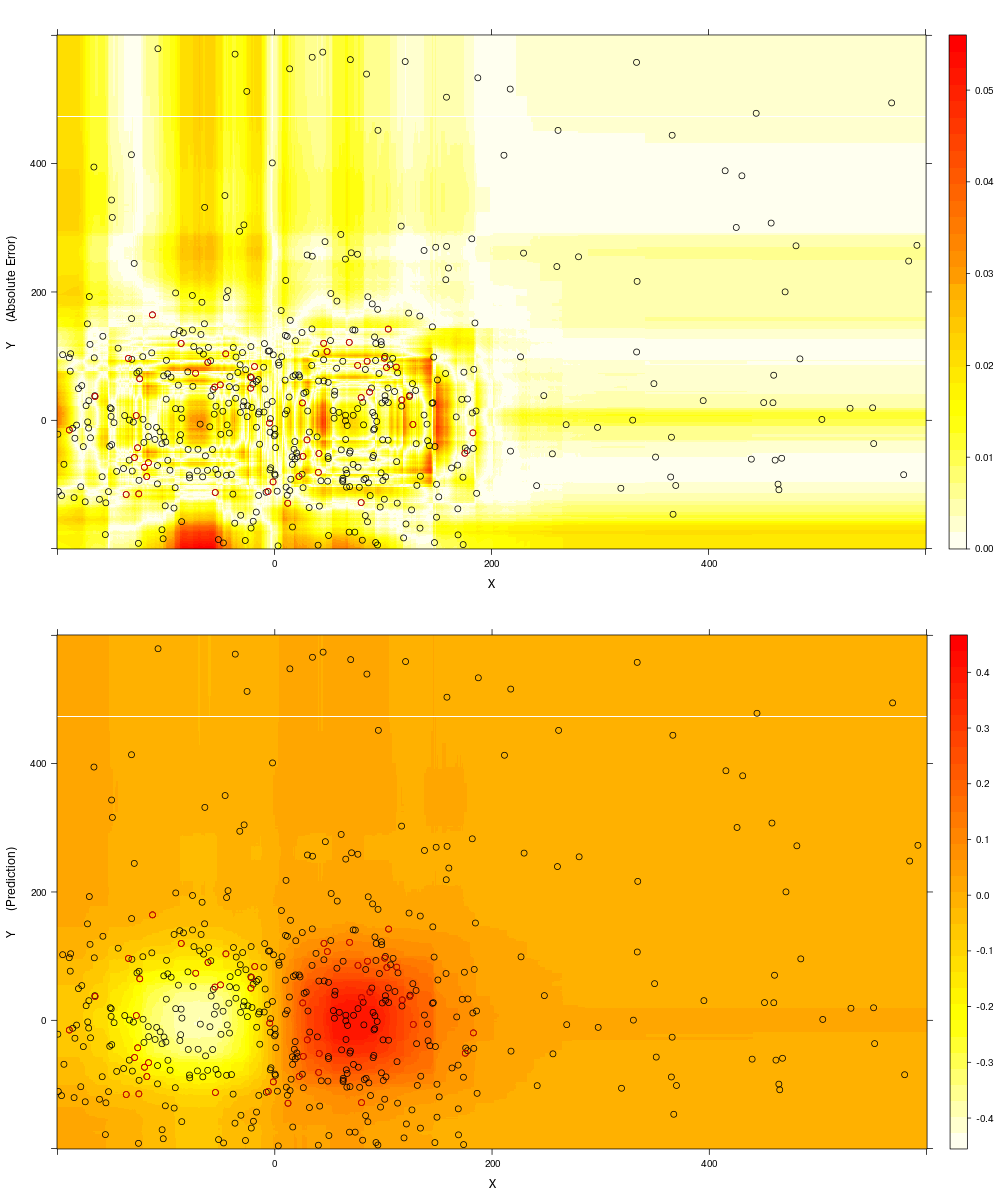
\includegraphics[width=\textwidth]{figures/ASK-gauss-levelplot.png}
\end{center}



The time series file contains the following values:
\begin{minted}{bash}
samples mean-error max-error rmse mean-relative max-relative
50 0.0377823384121497 0.447323111968324 0.0781095183475204 Inf Inf
100 0.0294159657374007 0.408494500075275 0.0630672408986823 Inf Inf
150 0.0275319895231202 0.281661273924844 0.0469645301362225 Inf Inf
200 0.0232192159241306 0.239290251332769 0.0376329805089173 Inf Inf
250 0.0174217850030764 0.142481821968832 0.0272243696109088 Inf Inf
300 0.0120016612421342 0.0846704149994422 0.0179698102164841 Inf Inf
350 0.00993725543490917 0.083600182129529 0.014940974890969 Inf Inf
400 0.00860058449418072 0.061942979615955 0.0124781071557198 Inf Inf
450 0.00835631286507885 0.0675461324475211 0.0126914309137798 Inf Inf
500 0.00787049320164634 0.0714181540783402 0.0119012098836963 Inf Inf
\end{minted}

The first column gives the number of samples; the following columns give the mean error of the model, the maximum error, the Root Mean Square Error (RMSE), the mean relative error, and the max relative error. The errors quantify the difference between the model prediction and the test set provided.
In this particular design space, since f can become 0, for example f(0,-200) = 0, the relative error is by definition undefined.

ASK includes a utility to plot the error time series:
\begin{minted}{bash}
$ <ask directory path>/utils/compare-time-series plot.png timeseries.out
\end{minted}

\begin{center}
  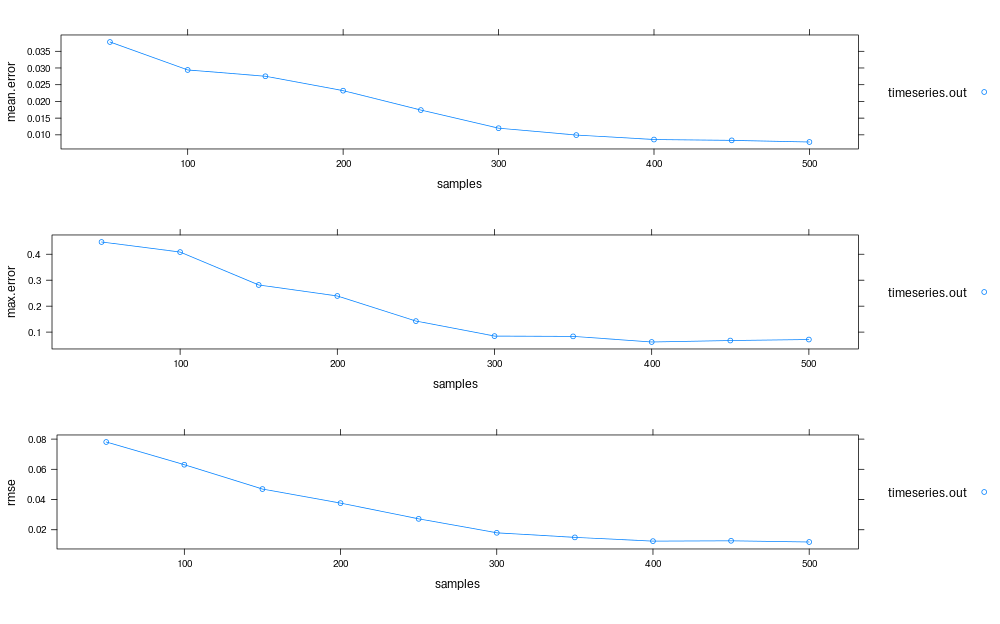
\includegraphics[width=\textwidth]{figures/ASK-gauss-timeseries.png}
\end{center}

The script is also useful to compare the accuracy of different configurations. Suppose different values are tried for the number of trees of the GBM model. For each configuration, experiments are rerun producing a new time series output \texttt{timeseries1.out, timeseries2.out, ...} 

Typing, 
\begin{minted}{bash}
$ <ask directory path>/utils/compare-time-series plot.png \
      timeseries1.out timeseries2.out [...]
\end{minted}

overlaps the error plots of each configuration.

Most sampling strategies included in ASK use random seeds. To evaluate precisely the behavior of one sampling strategy, it is recommended to take the median of multiple runs. The script \texttt{utils/merge-time-series} merges a set of individual time series by taking the median among all runs:
\begin{minted}{bash}
$ <ask directory path>/utils/merge-time-series aggregated.out \
      timeseries1.out timeseries2.out [...]
\end{minted}

\subsection{Reusing the Model}

Once ASK generates an accurate model, it can be used to predict any point in the exploration space. The model generated in the last iteration is \texttt{output/model00009.data}.

The model is able to predict the response for any new value. First, prepare a file with the desired combinations, for example:
\begin{minted}{bash}
<file: some.data>
10 10
50 -15.3
200 -30
\end{minted}

Then type:
\begin{minted}{bash}
$ export ASKHOME=<ask directory>; export PYTHONPATH=$ASKHOME:$PYTHONPATH
$ $ASKHOME/model/gbm_predict experiment.conf output/model00009.data \
    some.data prediction.data
$ cat prediction.data
10 10 0.098377986754355
50 -15.3 0.378151609613139
200 -30 0.0486711827411655
\end{minted}

Usually, the \texttt{ask} driver exports the two environment variables \texttt{ASKHOME} and \texttt{PYTHONPATH} automatically. In this example, the \texttt{gbm\_predict} module is called directly, therefore the two environment variables must be exported manually.

The predicted values can be compared with the true f values:

\begin{minted}{bash}
$  ./source.R experiment.conf some.data true.data
$ cat true.data
10 10 0.0980198673306755
50 -15.3 0.3803907821641490
200 -30 0.0334784671171613
\end{minted}

The prediction was very close for the first two points and less good for the last. 


\chapter{Standard Modules}
\section{Introduction}

This chapter presents the options for the standard modules bundled in ASK.

\section{Bootstrap Modules}

Bootstrap modules select the first batch of sampled points in the experiment.

\subsection{Module latinsquare}

Module latinsquare selects points using a Latin Hypercube sampling. The method is described in \emph{Large sample properties of simulations using Latin Hypercube Sampling}, M. Stein, Technometrics 1987, 143--151, JSTOR. ASK's module uses the \href{http://cran.r-project.org/web/packages/lhs/}{R lhs package} implementation.

	\vspace{0.5cm}\begin{tabular}{| p{0.18\textwidth} | p{0.18\textwidth} | p{0.14\textwidth} | p{0.50\textwidth}  |}
		\hline
		\textbf{ Parameters} & \textbf{ Mandatory} & \textbf{ Expects} & \textbf{ Description} \\ \hline
		 n &  yes &  integer &  Number of samples \\ \hline
		 method &   &  string: ``random'', ``genetic'' or ``maximin'' &  Method to generate the latin hypercube, refer to \href{http://cran.r-project.org/web/packages/lhs/}{lhs documentation} for details. ``random'' method is default. \\ \hline
		 seed &   &  integer &  Seed to initialize the Random Number Generator (RNG). When missing the default R RNG initialization is used. \\ \hline
	\end{tabular}

\subsection{Module lowdiscrepancy}

Module lowdiscrepancy selects points using a Low Discrepancy sequence. ASK's module uses the \href{http://cran.r-project.org/web/packages/fOptions/}{R fOptions package} implementation.

	\vspace{0.5cm}\begin{tabular}{| p{0.18\textwidth} | p{0.18\textwidth} | p{0.14\textwidth} | p{0.50\textwidth}  |}
		\hline
		\textbf{ Parameters} & \textbf{ Mandatory} & \textbf{ Expects} & \textbf{ Description} \\ \hline
		 n &  yes &  integer &  Number of samples \\ \hline
		 method &   &  string: ``sobol'' or ``halton'' &  Type of low discrepancy sequence, refer to \href{http://cran.r-project.org/web/packages/fOptions/}{fOptions documentation} for details. ``sobol'' method is default. \\ \hline
		 seed &   &  integer &  Seed to initialize the RNG. When missing the default R RNG initialization is used. \\ \hline
	\end{tabular}

\subsection{Module random}

Module random selects points by choosing a value for each factor using a uniform random distribution. 

	\vspace{0.5cm}\begin{tabular}{| p{0.18\textwidth} | p{0.18\textwidth} | p{0.14\textwidth} | p{0.50\textwidth}  |}
		\hline
		\textbf{ Parameters} & \textbf{ Mandatory} & \textbf{ Expects} & \textbf{ Description} \\ \hline
		 n &  yes &  integer & \\ \hline
		 seed &   &  integer &  Seed to initialize the RNG. When missing the default Python RNG initialization is used. \\ \hline
	\end{tabular}

\subsection{Module random-file}
/
Module random-file selects points by choosing samples at random from a samples file. The file must be in \hrefinternal{http:///wiki/Application\_Characterization:\_ASK:\_Chapter\_3:\_Experiment\_Setup\#Data\_Exchange\_Format}{ASK's data exchange format}.

	\vspace{0.5cm}\begin{tabular}{| p{0.18\textwidth} | p{0.18\textwidth} | p{0.14\textwidth} | p{0.50\textwidth}  |}
		\hline
		\textbf{ Parameters} & \textbf{ Mandatory} & \textbf{ Expects} & \textbf{ Description} \\ \hline
		 n &  yes &  integer &  Number of samples \\ \hline
		 data\_file &  yes &  path &  samples file \\ \hline
		 seed &   &  integer &  Seed to initialize the RNG. When missing the default Python RNG initialization is used. \\ \hline
	\end{tabular}

\section{Source Modules}

Source modules measure the samples selected by a bootstrap or sampler module. Usually, the user writes a custom source module fitting the target experiment.

\subsection{Module File}

The module file uses a text file as a database for returning measures. 
When the file module receives a requested set of samples, it tries to find them in the database file and returns the matching ones.

	\vspace{0.5cm}\begin{tabular}{| p{0.18\textwidth} | p{0.18\textwidth} | p{0.14\textwidth} | p{0.50\textwidth}  |}
		\hline
		\textbf{ Parameters} & \textbf{ Mandatory} & \textbf{ Expects} & \textbf{ Description} \\ \hline
		 data\_file &  yes &  path &  Path of the database file containing previously measured samples in \hrefinternal{http:///wiki/Application\_Characterization:\_ASK:\_Chapter\_3:\_Experiment\_Setup\#Data\_Exchange\_Format}{ASK's data exchange format}. \\ \hline
	\end{tabular}

\section{Sampler Modules}

The sampler module samples additional points in each iteration of the experimental pipeline. 

\subsection{Module amart}

Module amart selects points using the method described in \emph{Accurate and efficient processor performance prediction via regression tree based modeling}, B. Li and L. Peng and B. Ramadass, Journal of Systems Architecture 2009, 457--467. 

	\vspace{0.5cm}\begin{tabular}{| p{0.18\textwidth} | p{0.18\textwidth} | p{0.14\textwidth} | p{0.50\textwidth}  |}
		\hline
		\textbf{ Parameters} & \textbf{ Mandatory} & \textbf{ Expects} & \textbf{ Description} \\ \hline
		 n &  yes &  integer &  Number of samples \\ \hline
		 trees &   &  integer &  Number of trees used by the underlying GBM model. Default is 3000. \\ \hline
		 seeds &   &  integer &  Size of the committee. \\ \hline
		 predict\_on\_all &   &  boolean &  If true, the committee votes on all the candidate points. If false, the committee votes on a subsample of 20*n points using a Latin Hypercube sampling. Default is true. \\ \hline
	\end{tabular}

\subsection{Module hierarchical}

Module hierarchical selects points using the Hierarchical Variance Sampling method.

	\vspace{0.5cm}\begin{tabular}{| p{0.18\textwidth} | p{0.18\textwidth} | p{0.14\textwidth} | p{0.50\textwidth}  |}
		\hline
		\textbf{ Parameters} & \textbf{ Mandatory} & \textbf{ Expects} & \textbf{ Description} \\ \hline
		 n &  yes &  integer &  Number of samples \\ \hline
		 confidence &   &  float &  Confidence bound adjustment. A value of 0.9 means that the interval computed is valid 90\% of the time. Default is 0.9. \\ \hline
		 use\_cov &   &  boolean &  If true, the error per region is computed from the square of the coefficient of variance, also called relative variance. By default, it is false and the error is computed from the variance. \\ \hline
     use\_weights & & boolean & If true, a weights file is produced. It can be used by other modules (such as GBM) to compensate HVS uneven sampling during model construction. By default, it is true. \\ \hline
		 ponderate\_by\_size &   &  boolean &  If true, the error per region is defined as the square of the coefficient of variance multiplied by the region size. By default, it is true. \\ \hline
	\end{tabular}

\subsection{Module tgp}

Module tgp selects points using the \href{http://cran.r-project.org/web/packages/tgp/}{Tree Gaussian Process R package}. 

	\vspace{0.5cm}\begin{tabular}{| p{0.18\textwidth} | p{0.18\textwidth} | p{0.14\textwidth} | p{0.50\textwidth}  |}
		\hline
		\textbf{ Parameters} & \textbf{ Mandatory} & \textbf{ Expects} & \textbf{ Description} \\ \hline
		 n &  yes &  integer &  Number of samples \\ \hline
	\end{tabular}

\subsection{Module latinsquare}

Module latinsquare selects points using augmented Latin Hypercube samplings using the \href{http://cran.r-project.org/web/packages/lhs/}{lhs R package}.
If latinsquare is used as sampler, then latinsquare must be used as bootstrap.

	\vspace{0.5cm}\begin{tabular}{| p{0.18\textwidth} | p{0.18\textwidth} | p{0.14\textwidth} | p{0.50\textwidth}  |}
		\hline
		\textbf{ Parameters} & \textbf{ Mandatory} & \textbf{ Expects} & \textbf{ Description} \\ \hline
		 n &  yes &  integer &  Number of samples \\ \hline
	\end{tabular}

\subsection{Module random}

The random module selects points by choosing a value for each factor using a uniform random distribution. 
It also avoids selecting already sampled points.
When selecting an already sampled point, it discards the point and chooses a new random combination. 
The module finally gives up if, after 50 tries, it is unable to find a new combination, 

	\vspace{0.5cm}\begin{tabular}{| p{0.18\textwidth} | p{0.18\textwidth} | p{0.14\textwidth} | p{0.50\textwidth}  |}
		\hline
		\textbf{ Parameters} & \textbf{ Mandatory} & \textbf{ Expects} & \textbf{ Description} \\ \hline
		 n &  yes &  integer &  Number of samples \\ \hline
	\end{tabular}

\section{Model Modules}

Model modules predict the response in locations not yet sampled.

\subsection{Module cart}

Module cart uses the model described in \emph{CART: Classification and regression trees}, L. Breiman and J. Friedman and R. Olshen and C. Stone and D. Steinberg and P. Colla, Wadsworth 1983.

	\vspace{0.5cm}\begin{tabular}{| p{0.18\textwidth} | p{0.18\textwidth} | p{0.14\textwidth} | p{0.50\textwidth}  |}
		\hline
		\textbf{ Parameters} & \textbf{ Mandatory} & \textbf{ Expects} & \textbf{ Description} \\ \hline
		 cp &  yes &  float &  Complexity parameter \\ \hline
	\end{tabular}

\subsection{Module gbm}

Module gbm uses the model described in \href{http://cran.r-project.org/web/packages/gbm/}{\emph{Generalized Boosted Models: A guide to the gbm package}}, G. Ridgeway.

	\vspace{0.5cm}\begin{tabular}{| p{0.18\textwidth} | p{0.18\textwidth} | p{0.14\textwidth} | p{0.50\textwidth}  |}
		\hline
		\textbf{ Parameters} & \textbf{ Mandatory} & \textbf{ Expects} & \textbf{ Description} \\ \hline
		 ntreees &   &  integer &  Number of trees, default is 3000. \\ \hline
		 interactiondepth &   &  integer &  Interaction Depth, default is 8. \\ \hline
		 shrinkage &   &  float &  Shrinkage, default is 0.01 \\ \hline
		 distribution &   &  string: ``gaussian'', ``laplace'', for the full list check \href{http://cran.r-project.org/web/packages/gbm/}{gbm documentation}. &  Distribution function used when building the boosted tree model. Gaussian, the default minimizes RMSE error. Laplace minimizes the mean absolute error. \\ \hline
	\end{tabular}

\subsection{Module tgp}

Module tgp uses the Tree Gaussian Process model implemented in the \href{http://cran.r-project.org/web/packages/tgp/}{tgp R package}.

ASK's interface to the tgp module is not yet configurable.

\section{Control Modules}

Control modules choose when to end the experiment. 

\subsection{Module points}

Module points, stops the experiment after a fixed number of samples.

	\vspace{0.5cm}\begin{tabular}{| p{0.18\textwidth} | p{0.18\textwidth} | p{0.14\textwidth} | p{0.50\textwidth}  |}
		\hline
		\textbf{ Parameters} & \textbf{ Mandatory} & \textbf{ Expects} & \textbf{ Description} \\ \hline
		 n &  yes &  integer &  Number of samples. The experiment will be stopped when the number of points sampled reaches n. \\ \hline
	\end{tabular}

\subsection{Module convergence}

The module converge, stops the experiment if the model does not improve significantly in a given time window.
It computes the improvement on a measure of the model error. The accuracy values are read from a time series file. The timeseries file, which is briefly discussed in \hrefinternal{http:///wiki/Application\_Characterization:\_ASK:\_Chapter\_3:\_Experiment\_Setup\#Analyzing\_the\_experiment}{Chapter 3}, is composed of space separated values. 
The first line is a header with the name of the columns. The first column contains the number of
samples, the second column contain a measure of error. The file is automatically generated by
the \hrefinternal{http:///wiki/\#Module\_Generic}{generic reporter}, for example:

\begin{minted}{bash}
samples mean-error max-error rmse mean-relative max-relative
50 0.0377823384121497 0.447323111968324 0.0781095183475204 Inf Inf
100 0.0294159657374007 0.408494500075275 0.0630672408986823 Inf Inf
150 0.0275319895231202 0.281661273924844 0.0469645301362225 Inf Inf
\end{minted}

	\vspace{0.5cm}\begin{tabular}{| p{0.18\textwidth} | p{0.18\textwidth} | p{0.14\textwidth} | p{0.50\textwidth}  |}
		\hline
		\textbf{ Parameters} & \textbf{ Mandatory} & \textbf{ Expects} & \textbf{ Description} \\ \hline
		 timeseries &   &  path &  A file containing the model's error timeseries. If left empty, the module tries to retrieve the timeseries file from the report module configuration. \\ \hline
		 window &   &  int &  The window in number of iterations. The default value is 5. \\ \hline
		 threshold &   &  float &  Improvement threshold. A threshold of 0.1, means that if the error rate of change in the last \texttt{window} iterations is under 1\%, the experiment stops. \\ \hline
	\end{tabular}

\section{Reporter Modules}

Reporter modules produce informative statistics for the user during the experiment. 

\subsection{Module generic}

Module points, stops the experiment after a fixed number of samples.

	\vspace{0.5cm}\begin{tabular}{| p{0.18\textwidth} | p{0.18\textwidth} | p{0.14\textwidth} | p{0.50\textwidth}  |}
		\hline
		\textbf{ Parameters} & \textbf{ Mandatory} & \textbf{ Expects} & \textbf{ Description} \\ \hline
		 test\_set &  yes &  path &  File containing a set of samples. The model error is measured against this test-set of samples. The file must be in \hrefinternal{http:///wiki/\#Data_Exchange_Format}{ASK's data exchange format}. \\ \hline
		 script &  yes &  path: ``reporter/generic/1D.R'' or ``reporter/generic/2D.R'' or user provided script &  This is the path of the script used for plotting the model's predictions. This module includes generic scripts for 1D and 2D design spaces, that is to say composed of one or two factors. For higher-dimension spaces, the user must \hrefinternal{http:///wiki/Application_Characterization:_ASK:_Chapter_5:_Writing_Modules}{write a custom reporter}. \\ \hline
		 timeseries &   &  path &  Path of the time series file. Error measures of the model will be written to this file. \\ \hline
		 max\_error\_scale &   &  float &  If specified, it represents the error's plot maximal error value. If left empty, the error's plot range is dynamically adapted. \\ \hline
	\end{tabular}



\chapter{Writing Modules}
\section{Introduction}

The following chapter presents the \hrefinternal{http:///wiki/\#Modules_Interfaces}{modules interfaces} and explains \hrefinternal{http:///wiki/\#Writing_Custom_Modules}{how to write custom modules} for ASK.

\section{Module Interfaces}

Each kind of module has a strictly defined interface. For instance, every source module expects one configuration, one input and one output file.
This design makes possible to use as a source module any module implementation adhering to its interface. 
This section describes the interface for each kind of module.

Except if noted otherwise, each time a file is used in the modules below the format must be in ASK's \hrefinternal{http:///wiki/Application\_Characterization:_ASK:_Chapter_3:_Experiment_Setup\#Data_Exchange_Format}{data exchange format}.

\subsection{Bootstrap Interface}

A Bootstrap module selects the initial batch of points measured by ASK.

\emph{Interface:} \texttt{bootstrap \textless{}configuration\textgreater{} \textless{}output\_file\textgreater{}} 

\emph{Input:}
\begin{itemize}
	\item \texttt{configuration}: ASK configuration file
\end{itemize}

\emph{Output:}
\begin{itemize}
	\item \texttt{output\_file}: path of the output file. The output file contains a list of requested factors to be measured; therefore, it has no response column.
\end{itemize}

\subsection{Source Interface}

A source module computes the actual measures for the requested factors and returns the response.

\emph{Interface:} \texttt{source \textless{}configuration\textgreater{} \textless{}requested\_file\textgreater{} \textless{}output\_file\textgreater{}} 

\emph{Input:}
\begin{itemize}
	\item \texttt{configuration}: ASK configuration file
	\item \texttt{requested\_file}: path of the requested file containing the factors, which need to be measured
\end{itemize}

\emph{Output:}
\begin{itemize}
	\item \texttt{output\_file}: path of the output file. The output must include the factors passed on the requested file with an additional column containing the measured response for each factor combination.
\end{itemize}

\subsection{Model Interface}

A Model module builds a surrogate model for the experiment on the sampled points. It builds a function that predicts the response for every factor combination. The model predicts the unknown points, that is to say, the not measured ones.
Model modules are special, in that their output is module dependent. For instance, the GBM model produces General Boosted Models, the TGP model produces Tree Gaussian Process models. All the model modules distributed within ASK come in two parts:

\begin{itemize}
	\item model\_build, which allows to build the model
	\item model\_predict, which allows to use the model to predict unknown points
\end{itemize}

\emph{Interface:} \texttt{model\_build \textless{}configuration\textgreater{} \textless{}labelled\_file\textgreater{} \textless{}output\_file\textgreater{}} 

\emph{Input:}
\begin{itemize}
	\item \texttt{configuration}: ASK configuration file
	\item \texttt{labelled\_file}: path of the labelled file containing a list of measured points. It therefore contains factors columns and a response column.
\end{itemize}

\emph{Output:}
\begin{itemize}
	\item \texttt{output\_file}: path of the output file. The output file format depends on the module, it may be or may not be in ASK's \hrefinternal{http:///wiki/Application\_Characterization:_ASK:_Chapter_3:_Experiment_Setup\#Data_Exchange_Format}{data exchange format}. The output file contains the built model.
\end{itemize}

\emph{Interface:} \texttt{model\_predict \textless{}configuration.conf\textgreater{} \textless{}model\textgreater{} \textless{}requested\_file\textgreater{} \textless{}output\_file\textgreater{}} 

\emph{Input:}
\begin{itemize}
	\item \texttt{configuration}: ASK configuration file
	\item \texttt{model\_file}: path of the model file, produced by the associated \texttt{model\_build} command
	\item \texttt{requested\_file}: path of the labelled file containing a list of points to predict, therefore the response column is missing
\end{itemize}

\emph{Output:}
\begin{itemize}
	\item \texttt{output\_file}: path of the output file. The output file contains the same points passed in the requested\_file with a response column filled with the model's predictions.
\end{itemize}

\subsection{Sampler Interface}

A Sampler module selects a new batch of points to measure for every iteration after the first.
Bootstrap modules are in charge of selecting the first iteration's batch of points.

\emph{Interface:} \texttt{sampler \textless{}configuration\textgreater{} \textless{}input\_file\textgreater{} \textless{}output\_file\textgreater{}} 

\emph{Input:}
\begin{itemize}
	\item \texttt{configuration}: ASK configuration file
	\item \texttt{input\_file}: path of the input file containing the points that have already been measured an a column with their responses
\end{itemize}

\emph{Output:}
\begin{itemize}
	\item \texttt{output\_file}: path of the output file containing the new list of points to measure; therefore, it has no response column
\end{itemize}

\subsection{Control Interface}

A Control module decides when the sampling process ends. Two basic strategies are included in ASK: stopping when a predefined amount of points has been sampled or stopping when the accuracy improvement stays under a given threshold for a number of iterations.

\emph{Interface:} \texttt{points \textless{}configuration\textgreater{} \textless{}labelled\_file\textgreater{} \textless{}model\_file\textgreater{}} 

\emph{Input:}
\begin{itemize}
	\item \texttt{configuration}: ASK configuration file
	\item \texttt{labelled\_file}: path of the labelled file. It contains the points that have already been measured, it has a response column
	\item \texttt{model\_file}: path of the model file generated by the model module
\end{itemize}

\emph{Output:}
\begin{itemize}
	\item Control modules should return exit code 254 to stop the experiment, or any other code to pursue the experiment.
\end{itemize}

\subsection{Reporter Interface}

A Reporter module produces detailed statistics about the sampling.

\emph{Interface:} \texttt{reporter \textless{}configuration\textgreater{} \textless{}iteration\textgreater{} \textless{}labelled\_file\textgreater{} \textless{}newly\_labelled\_file\textgreater{} \textless{}model\_file\textgreater{}} 

\emph{Input:}
\begin{itemize}
	\item \texttt{configuration}: ASK configuration file
	\item \texttt{iteration}: iteration number, the bootstrap iteration is numbered 0
	\item \texttt{labelled\_file}: path of the labelled file containing the points that have already been measured, it has a response column
	\item \texttt{newly\_labelled\_file}: path of the newly labelled file containing the points that have been measured in the last iteration, it has a response column
	\item \texttt{model\_file}: path of the model file generated by the model module
\end{itemize}

\emph{Output:}
\begin{itemize}
	\item None required.
\end{itemize}

\section{Writing Custom Modules}

Custom modules may be written in any chosen language as long as they adhere to the \hrefinternal{http:///wiki/\#Module_interfaces}{module interfaces}.
As an example, the following section shows how to design a simple bootstrap module baptized Grid.

The grid module selects points regularly distributed in a grid. To make things simpler, it will only work with integer factors. The module is written in Python.

The grid module takes one parameter, \texttt{grid\_size}, which is the grid size. 
Supposing the design space has two factors x and y varying between 0 and 10, a grid size of 2 will select points (0,0), (0,2), (0,4) ... (0,10), (2,0), (2,2) ... (10,10).

\subsection{Input Parser}

The first step is writing a parser adhering to the \hrefinternal{http:///wiki/\#Bootstrap_Interface}{bootstrap interface}:
\begin{minted}{bash}
bootstrap <configuration> <output_file>
\end{minted}

In the example, the argparse module will be used:

\begin{minted}{python}
#!/usr/bin/env python
if __name__ == "__main__":
  import argparse
  parser = argparse.ArgumentParser(description="Sample the design space in a" 
             " grid fashion")
  parser.add_argument("configuration")
  parser.add_argument("output_file")
  args = parser.parse_args()
\end{minted}

After parsing the command line arguments, the module needs to parse the configuration file. ASK already provides a library for this purpose in python and in R.

\begin{minted}{python}
from common.configuration import Configuration
conf = Configuration(args.configuration)
\end{minted}

The conf object can be used to retrieve configurations values. To retrieve the \texttt{grid\_size} parameter, one can use:
\begin{minted}{python}
grid_size = conf("modules.bootstrap.params.grid_size")
\end{minted}

In the above code, if the parameter is missing, or is of the wrong type, the module fails and an error is logged. Fortunately, the conf object handles type checking and default values substituting the above code with:

\begin{minted}{python}
grid_size = conf("modules.bootstrap.params.grid_size", int, 1)
\end{minted}

Now, if the parameter is of the wrong type, an appropriate message is raised. Moreover, if the \texttt{grid\_size} parameter is missing, the default 1 value is used. 

Then the module retrieves the factors's configuration and checks that only integer factors were used:

\begin{minted}{python}
from common.util import fatal
factors = conf("factors")
for f in factors:
   if f["type"] != "integer":
     fatal("Grid bootstrap only works with integer factors.")
\end{minted}

Finally, pass all the input information to an appropriate function:
\begin{minted}{python}
grid_bootstrap(args.output_file, grid_size, factors)
\end{minted}

\subsection{Bootstrap Logic}

The previous code ensures that all the arguments are correctly parsed and strictly adheres to the \hrefinternal{http:///wiki/\#Bootstrap_Interface}{bootstrap interface}.
All that remains is writing the logic of the module. First, for each factor, the list of values in the grid is computed.

\begin{minted}{python}
def grid_bootstrap(output, grid_size, factors):
  from itertools import product
  coords = []
  for f in factors:
      coords.append(xrange(f["range"]["min"], f["range"]["max"] + 1, grid_size))
\end{minted}

Then, the module computes a Cartesian product of the previous values and writes the coordinates in \hrefinternal{http:///wiki/Application\_Characterization:_ASK:_Chapter_3:_Experiment_Setup\#Data_Exchange_Format}{ASK's data exchange format}:

\begin{minted}{python}
  out = file(output, "w")
  for c in product(*coords):
      out.write(" ".join(map(str,c)) + "\n")
  out.close()
\end{minted}

The custom module is now complete. It can be used as a drop-in replacement for an existing bootstrap module.
For example, changing the bootstrap module to ``grid'' inside \texttt{examples/face/experiment.conf} with a grid\_size of 20, produces the following report:

\begin{center}
  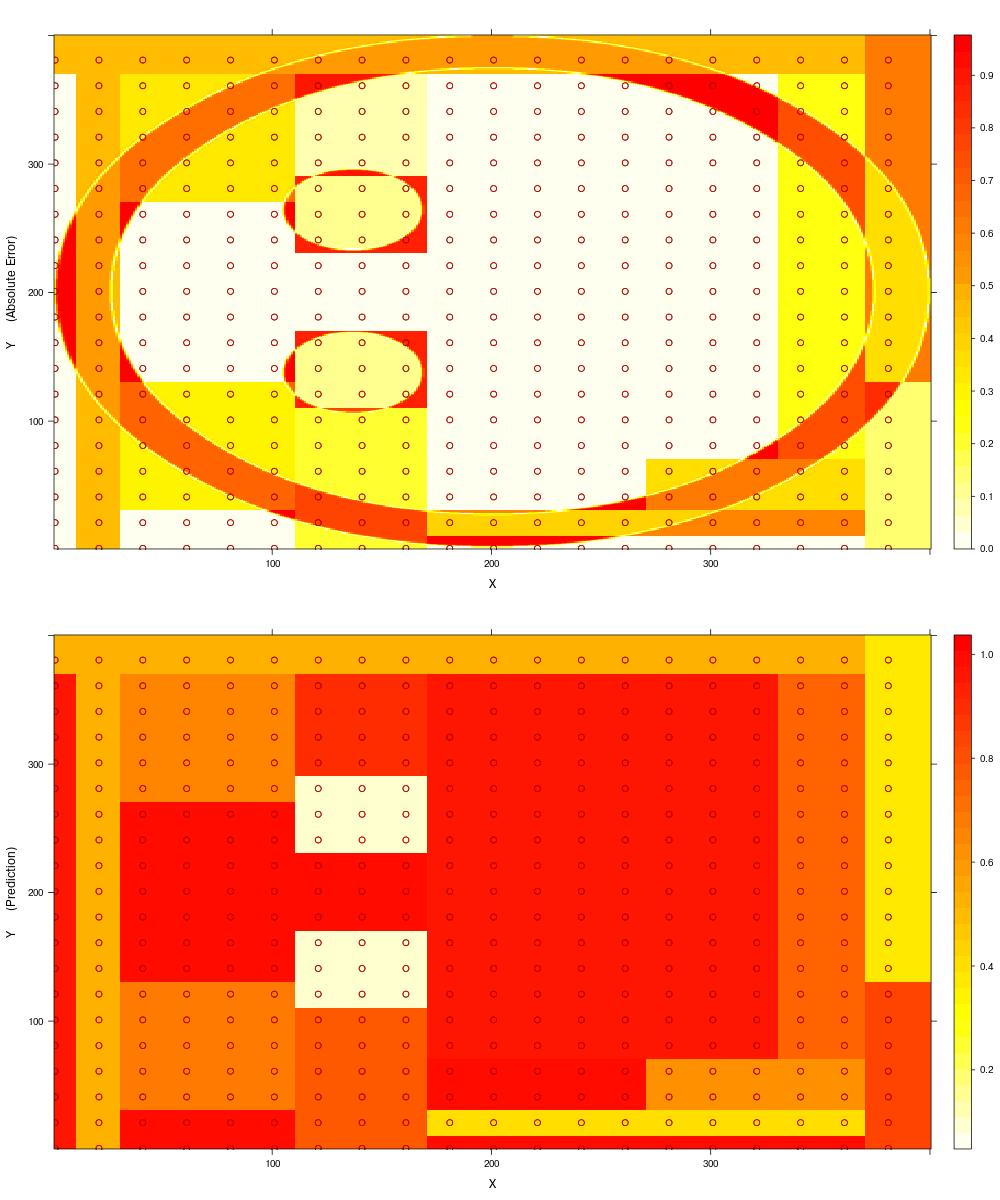
\includegraphics[width=\textwidth]{figures/ASK-Custom-Grid.png}
\end{center}



\chapter{Support}
\section{Issues and Features}

Google code provides a bug tracker on project pages. Users and developers can write new issues or features, called tickets, at \href{http://code.google.com/p/adaptive-sampling-kit/issues/list}{ASK bug tracker}. To open tickets please follow the rules below.

\subsection{Program Bugs}

The following steps should be used to open a bug ticket:

\begin{enumerate}
	\item Template: Choose Defect request from user or developer, accordingly.
	\item Subject: Choose an explicit title, summarizing the issue.
	\item Description: Add a brief abstract of the bug. Describe the exact steps that triggered the bug, and if possible attach the files needed to reproduce it.
\end{enumerate}

\subsection{Feature Requests}

The following steps should be used to open a feature ticket:

\begin{enumerate}
	\item Tracker: Choose ``Review request.''
	\item Subject: Choose an explicit title, summarizing the issue.
	\item Description: Add a description of the feature.
\end{enumerate}

\section{Contributing}

The project is particularly interested in:
\begin{itemize}
	\item Patches fixing bugs or adding new features
	\item Documentation fixes
	\item Bug reports
\end{itemize}

For documentation fixes and bug reports, please use the \href{http://code.google.com/p/adaptive-sampling-kit/issues/list}{issue tracker}.
For code contributions, contact us at \textbf{\href{mailto:ask-team@exascale-computing.eu}{ask-team@exascale-computing.eu}}.

\subsection{Running the Test Suite}

ASK comes with an extensive suite of tests. Before submitting a patch, please make sure that all the tests pass, with the following command:
\begin{minted}{bash}
cd tests/
nosetests -v
\end{minted}

If you submit a patch, including unit tests for your code is more than welcome and will make the patch review faster.

\chapter*{GNU Free Documentation License}
\phantomsection  % so hyperref creates bookmarks
\addcontentsline{toc}{chapter}{GNU Free Documentation License}
%\label{label_fdl}

 \begin{center}

       Version 1.3, 3 November 2008


 Copyright \copyright{} 2000, 2001, 2002, 2007, 2008  Free Software Foundation, Inc.
 
 \bigskip
 
     \texttt{<http://fsf.org/>}
  
 \bigskip
 
 Everyone is permitted to copy and distribute verbatim copies
 of this license document, but changing it is not allowed.
\end{center}


\begin{center}
{\bf\large Preamble}
\end{center}

The purpose of this License is to make a manual, textbook, or other
functional and useful document ``free'' in the sense of freedom: to
assure everyone the effective freedom to copy and redistribute it,
with or without modifying it, either commercially or noncommercially.
Secondarily, this License preserves for the author and publisher a way
to get credit for their work, while not being considered responsible
for modifications made by others.

This License is a kind of ``copyleft'', which means that derivative
works of the document must themselves be free in the same sense.  It
complements the GNU General Public License, which is a copyleft
license designed for free software.

We have designed this License in order to use it for manuals for free
software, because free software needs free documentation: a free
program should come with manuals providing the same freedoms that the
software does.  But this License is not limited to software manuals;
it can be used for any textual work, regardless of subject matter or
whether it is published as a printed book.  We recommend this License
principally for works whose purpose is instruction or reference.


\begin{center}
{\Large\bf 1. APPLICABILITY AND DEFINITIONS\par}
\phantomsection
\addcontentsline{toc}{section}{1. APPLICABILITY AND DEFINITIONS}
\end{center}

This License applies to any manual or other work, in any medium, that
contains a notice placed by the copyright holder saying it can be
distributed under the terms of this License.  Such a notice grants a
world-wide, royalty-free license, unlimited in duration, to use that
work under the conditions stated herein.  The ``\textbf{Document}'', below,
refers to any such manual or work.  Any member of the public is a
licensee, and is addressed as ``\textbf{you}''.  You accept the license if you
copy, modify or distribute the work in a way requiring permission
under copyright law.

A ``\textbf{Modified Version}'' of the Document means any work containing the
Document or a portion of it, either copied verbatim, or with
modifications and/or translated into another language.

A ``\textbf{Secondary Section}'' is a named appendix or a front-matter section of
the Document that deals exclusively with the relationship of the
publishers or authors of the Document to the Document's overall subject
(or to related matters) and contains nothing that could fall directly
within that overall subject.  (Thus, if the Document is in part a
textbook of mathematics, a Secondary Section may not explain any
mathematics.)  The relationship could be a matter of historical
connection with the subject or with related matters, or of legal,
commercial, philosophical, ethical or political position regarding
them.

The ``\textbf{Invariant Sections}'' are certain Secondary Sections whose titles
are designated, as being those of Invariant Sections, in the notice
that says that the Document is released under this License.  If a
section does not fit the above definition of Secondary then it is not
allowed to be designated as Invariant.  The Document may contain zero
Invariant Sections.  If the Document does not identify any Invariant
Sections then there are none.

The ``\textbf{Cover Texts}'' are certain short passages of text that are listed,
as Front-Cover Texts or Back-Cover Texts, in the notice that says that
the Document is released under this License.  A Front-Cover Text may
be at most 5 words, and a Back-Cover Text may be at most 25 words.

A ``\textbf{Transparent}'' copy of the Document means a machine-readable copy,
represented in a format whose specification is available to the
general public, that is suitable for revising the document
straightforwardly with generic text editors or (for images composed of
pixels) generic paint programs or (for drawings) some widely available
drawing editor, and that is suitable for input to text formatters or
for automatic translation to a variety of formats suitable for input
to text formatters.  A copy made in an otherwise Transparent file
format whose markup, or absence of markup, has been arranged to thwart
or discourage subsequent modification by readers is not Transparent.
An image format is not Transparent if used for any substantial amount
of text.  A copy that is not ``Transparent'' is called ``\textbf{Opaque}''.

Examples of suitable formats for Transparent copies include plain
ASCII without markup, Texinfo input format, LaTeX input format, SGML
or XML using a publicly available DTD, and standard-conforming simple
HTML, PostScript or PDF designed for human modification.  Examples of
transparent image formats include PNG, XCF and JPG.  Opaque formats
include proprietary formats that can be read and edited only by
proprietary word processors, SGML or XML for which the DTD and/or
processing tools are not generally available, and the
machine-generated HTML, PostScript or PDF produced by some word
processors for output purposes only.

The ``\textbf{Title Page}'' means, for a printed book, the title page itself,
plus such following pages as are needed to hold, legibly, the material
this License requires to appear in the title page.  For works in
formats which do not have any title page as such, ``Title Page'' means
the text near the most prominent appearance of the work's title,
preceding the beginning of the body of the text.

The ``\textbf{publisher}'' means any person or entity that distributes
copies of the Document to the public.

A section ``\textbf{Entitled XYZ}'' means a named subunit of the Document whose
title either is precisely XYZ or contains XYZ in parentheses following
text that translates XYZ in another language.  (Here XYZ stands for a
specific section name mentioned below, such as ``\textbf{Acknowledgements}'',
``\textbf{Dedications}'', ``\textbf{Endorsements}'', or ``\textbf{History}''.)  
To ``\textbf{Preserve the Title}''
of such a section when you modify the Document means that it remains a
section ``Entitled XYZ'' according to this definition.

The Document may include Warranty Disclaimers next to the notice which
states that this License applies to the Document.  These Warranty
Disclaimers are considered to be included by reference in this
License, but only as regards disclaiming warranties: any other
implication that these Warranty Disclaimers may have is void and has
no effect on the meaning of this License.


\begin{center}
{\Large\bf 2. VERBATIM COPYING\par}
\phantomsection
\addcontentsline{toc}{section}{2. VERBATIM COPYING}
\end{center}

You may copy and distribute the Document in any medium, either
commercially or noncommercially, provided that this License, the
copyright notices, and the license notice saying this License applies
to the Document are reproduced in all copies, and that you add no other
conditions whatsoever to those of this License.  You may not use
technical measures to obstruct or control the reading or further
copying of the copies you make or distribute.  However, you may accept
compensation in exchange for copies.  If you distribute a large enough
number of copies you must also follow the conditions in section~3.

You may also lend copies, under the same conditions stated above, and
you may publicly display copies.


\begin{center}
{\Large\bf 3. COPYING IN QUANTITY\par}
\phantomsection
\addcontentsline{toc}{section}{3. COPYING IN QUANTITY}
\end{center}


If you publish printed copies (or copies in media that commonly have
printed covers) of the Document, numbering more than 100, and the
Document's license notice requires Cover Texts, you must enclose the
copies in covers that carry, clearly and legibly, all these Cover
Texts: Front-Cover Texts on the front cover, and Back-Cover Texts on
the back cover.  Both covers must also clearly and legibly identify
you as the publisher of these copies.  The front cover must present
the full title with all words of the title equally prominent and
visible.  You may add other material on the covers in addition.
Copying with changes limited to the covers, as long as they preserve
the title of the Document and satisfy these conditions, can be treated
as verbatim copying in other respects.

If the required texts for either cover are too voluminous to fit
legibly, you should put the first ones listed (as many as fit
reasonably) on the actual cover, and continue the rest onto adjacent
pages.

If you publish or distribute Opaque copies of the Document numbering
more than 100, you must either include a machine-readable Transparent
copy along with each Opaque copy, or state in or with each Opaque copy
a computer-network location from which the general network-using
public has access to download using public-standard network protocols
a complete Transparent copy of the Document, free of added material.
If you use the latter option, you must take reasonably prudent steps,
when you begin distribution of Opaque copies in quantity, to ensure
that this Transparent copy will remain thus accessible at the stated
location until at least one year after the last time you distribute an
Opaque copy (directly or through your agents or retailers) of that
edition to the public.

It is requested, but not required, that you contact the authors of the
Document well before redistributing any large number of copies, to give
them a chance to provide you with an updated version of the Document.


\begin{center}
{\Large\bf 4. MODIFICATIONS\par}
\phantomsection
\addcontentsline{toc}{section}{4. MODIFICATIONS}
\end{center}

You may copy and distribute a Modified Version of the Document under
the conditions of sections 2 and 3 above, provided that you release
the Modified Version under precisely this License, with the Modified
Version filling the role of the Document, thus licensing distribution
and modification of the Modified Version to whoever possesses a copy
of it.  In addition, you must do these things in the Modified Version:

\begin{itemize}
\item[A.] 
   Use in the Title Page (and on the covers, if any) a title distinct
   from that of the Document, and from those of previous versions
   (which should, if there were any, be listed in the History section
   of the Document).  You may use the same title as a previous version
   if the original publisher of that version gives permission.
   
\item[B.]
   List on the Title Page, as authors, one or more persons or entities
   responsible for authorship of the modifications in the Modified
   Version, together with at least five of the principal authors of the
   Document (all of its principal authors, if it has fewer than five),
   unless they release you from this requirement.
   
\item[C.]
   State on the Title page the name of the publisher of the
   Modified Version, as the publisher.
   
\item[D.]
   Preserve all the copyright notices of the Document.
   
\item[E.]
   Add an appropriate copyright notice for your modifications
   adjacent to the other copyright notices.
   
\item[F.]
   Include, immediately after the copyright notices, a license notice
   giving the public permission to use the Modified Version under the
   terms of this License, in the form shown in the Addendum below.
   
\item[G.]
   Preserve in that license notice the full lists of Invariant Sections
   and required Cover Texts given in the Document's license notice.
   
\item[H.]
   Include an unaltered copy of this License.
   
\item[I.]
   Preserve the section Entitled ``History'', Preserve its Title, and add
   to it an item stating at least the title, year, new authors, and
   publisher of the Modified Version as given on the Title Page.  If
   there is no section Entitled ``History'' in the Document, create one
   stating the title, year, authors, and publisher of the Document as
   given on its Title Page, then add an item describing the Modified
   Version as stated in the previous sentence.
   
\item[J.]
   Preserve the network location, if any, given in the Document for
   public access to a Transparent copy of the Document, and likewise
   the network locations given in the Document for previous versions
   it was based on.  These may be placed in the ``History'' section.
   You may omit a network location for a work that was published at
   least four years before the Document itself, or if the original
   publisher of the version it refers to gives permission.
   
\item[K.]
   For any section Entitled ``Acknowledgements'' or ``Dedications'',
   Preserve the Title of the section, and preserve in the section all
   the substance and tone of each of the contributor acknowledgements
   and/or dedications given therein.
   
\item[L.]
   Preserve all the Invariant Sections of the Document,
   unaltered in their text and in their titles.  Section numbers
   or the equivalent are not considered part of the section titles.
   
\item[M.]
   Delete any section Entitled ``Endorsements''.  Such a section
   may not be included in the Modified Version.
   
\item[N.]
   Do not retitle any existing section to be Entitled ``Endorsements''
   or to conflict in title with any Invariant Section.
   
\item[O.]
   Preserve any Warranty Disclaimers.
\end{itemize}

If the Modified Version includes new front-matter sections or
appendices that qualify as Secondary Sections and contain no material
copied from the Document, you may at your option designate some or all
of these sections as invariant.  To do this, add their titles to the
list of Invariant Sections in the Modified Version's license notice.
These titles must be distinct from any other section titles.

You may add a section Entitled ``Endorsements'', provided it contains
nothing but endorsements of your Modified Version by various
parties---for example, statements of peer review or that the text has
been approved by an organization as the authoritative definition of a
standard.

You may add a passage of up to five words as a Front-Cover Text, and a
passage of up to 25 words as a Back-Cover Text, to the end of the list
of Cover Texts in the Modified Version.  Only one passage of
Front-Cover Text and one of Back-Cover Text may be added by (or
through arrangements made by) any one entity.  If the Document already
includes a cover text for the same cover, previously added by you or
by arrangement made by the same entity you are acting on behalf of,
you may not add another; but you may replace the old one, on explicit
permission from the previous publisher that added the old one.

The author(s) and publisher(s) of the Document do not by this License
give permission to use their names for publicity for or to assert or
imply endorsement of any Modified Version.


\begin{center}
{\Large\bf 5. COMBINING DOCUMENTS\par}
\phantomsection
\addcontentsline{toc}{section}{5. COMBINING DOCUMENTS}
\end{center}


You may combine the Document with other documents released under this
License, under the terms defined in section~4 above for modified
versions, provided that you include in the combination all of the
Invariant Sections of all of the original documents, unmodified, and
list them all as Invariant Sections of your combined work in its
license notice, and that you preserve all their Warranty Disclaimers.

The combined work need only contain one copy of this License, and
multiple identical Invariant Sections may be replaced with a single
copy.  If there are multiple Invariant Sections with the same name but
different contents, make the title of each such section unique by
adding at the end of it, in parentheses, the name of the original
author or publisher of that section if known, or else a unique number.
Make the same adjustment to the section titles in the list of
Invariant Sections in the license notice of the combined work.

In the combination, you must combine any sections Entitled ``History''
in the various original documents, forming one section Entitled
``History''; likewise combine any sections Entitled ``Acknowledgements'',
and any sections Entitled ``Dedications''.  You must delete all sections
Entitled ``Endorsements''.

\begin{center}
{\Large\bf 6. COLLECTIONS OF DOCUMENTS\par}
\phantomsection
\addcontentsline{toc}{section}{6. COLLECTIONS OF DOCUMENTS}
\end{center}

You may make a collection consisting of the Document and other documents
released under this License, and replace the individual copies of this
License in the various documents with a single copy that is included in
the collection, provided that you follow the rules of this License for
verbatim copying of each of the documents in all other respects.

You may extract a single document from such a collection, and distribute
it individually under this License, provided you insert a copy of this
License into the extracted document, and follow this License in all
other respects regarding verbatim copying of that document.


\begin{center}
{\Large\bf 7. AGGREGATION WITH INDEPENDENT WORKS\par}
\phantomsection
\addcontentsline{toc}{section}{7. AGGREGATION WITH INDEPENDENT WORKS}
\end{center}


A compilation of the Document or its derivatives with other separate
and independent documents or works, in or on a volume of a storage or
distribution medium, is called an ``aggregate'' if the copyright
resulting from the compilation is not used to limit the legal rights
of the compilation's users beyond what the individual works permit.
When the Document is included in an aggregate, this License does not
apply to the other works in the aggregate which are not themselves
derivative works of the Document.

If the Cover Text requirement of section~3 is applicable to these
copies of the Document, then if the Document is less than one half of
the entire aggregate, the Document's Cover Texts may be placed on
covers that bracket the Document within the aggregate, or the
electronic equivalent of covers if the Document is in electronic form.
Otherwise they must appear on printed covers that bracket the whole
aggregate.


\begin{center}
{\Large\bf 8. TRANSLATION\par}
\phantomsection
\addcontentsline{toc}{section}{8. TRANSLATION}
\end{center}


Translation is considered a kind of modification, so you may
distribute translations of the Document under the terms of section~4.
Replacing Invariant Sections with translations requires special
permission from their copyright holders, but you may include
translations of some or all Invariant Sections in addition to the
original versions of these Invariant Sections.  You may include a
translation of this License, and all the license notices in the
Document, and any Warranty Disclaimers, provided that you also include
the original English version of this License and the original versions
of those notices and disclaimers.  In case of a disagreement between
the translation and the original version of this License or a notice
or disclaimer, the original version will prevail.

If a section in the Document is Entitled ``Acknowledgements'',
``Dedications'', or ``History'', the requirement (section~4) to Preserve
its Title (section~1) will typically require changing the actual
title.


\begin{center}
{\Large\bf 9. TERMINATION\par}
\phantomsection
\addcontentsline{toc}{section}{9. TERMINATION}
\end{center}


You may not copy, modify, sublicense, or distribute the Document
except as expressly provided under this License.  Any attempt
otherwise to copy, modify, sublicense, or distribute it is void, and
will automatically terminate your rights under this License.

However, if you cease all violation of this License, then your license
from a particular copyright holder is reinstated (a) provisionally,
unless and until the copyright holder explicitly and finally
terminates your license, and (b) permanently, if the copyright holder
fails to notify you of the violation by some reasonable means prior to
60 days after the cessation.

Moreover, your license from a particular copyright holder is
reinstated permanently if the copyright holder notifies you of the
violation by some reasonable means, this is the first time you have
received notice of violation of this License (for any work) from that
copyright holder, and you cure the violation prior to 30 days after
your receipt of the notice.

Termination of your rights under this section does not terminate the
licenses of parties who have received copies or rights from you under
this License.  If your rights have been terminated and not permanently
reinstated, receipt of a copy of some or all of the same material does
not give you any rights to use it.


\begin{center}
{\Large\bf 10. FUTURE REVISIONS OF THIS LICENSE\par}
\phantomsection
\addcontentsline{toc}{section}{10. FUTURE REVISIONS OF THIS LICENSE}
\end{center}


The Free Software Foundation may publish new, revised versions
of the GNU Free Documentation License from time to time.  Such new
versions will be similar in spirit to the present version, but may
differ in detail to address new problems or concerns.  See
\texttt{http://www.gnu.org/copyleft/}.

Each version of the License is given a distinguishing version number.
If the Document specifies that a particular numbered version of this
License ``or any later version'' applies to it, you have the option of
following the terms and conditions either of that specified version or
of any later version that has been published (not as a draft) by the
Free Software Foundation.  If the Document does not specify a version
number of this License, you may choose any version ever published (not
as a draft) by the Free Software Foundation.  If the Document
specifies that a proxy can decide which future versions of this
License can be used, that proxy's public statement of acceptance of a
version permanently authorizes you to choose that version for the
Document.


\begin{center}
{\Large\bf 11. RELICENSING\par}
\phantomsection
\addcontentsline{toc}{section}{11. RELICENSING}
\end{center}


``Massive Multiauthor Collaboration Site'' (or ``MMC Site'') means any
World Wide Web server that publishes copyrightable works and also
provides prominent facilities for anybody to edit those works.  A
public wiki that anybody can edit is an example of such a server.  A
``Massive Multiauthor Collaboration'' (or ``MMC'') contained in the
site means any set of copyrightable works thus published on the MMC
site.

``CC-BY-SA'' means the Creative Commons Attribution-Share Alike 3.0
license published by Creative Commons Corporation, a not-for-profit
corporation with a principal place of business in San Francisco,
California, as well as future copyleft versions of that license
published by that same organization.

``Incorporate'' means to publish or republish a Document, in whole or
in part, as part of another Document.

An MMC is ``eligible for relicensing'' if it is licensed under this
License, and if all works that were first published under this License
somewhere other than this MMC, and subsequently incorporated in whole
or in part into the MMC, (1) had no cover texts or invariant sections,
and (2) were thus incorporated prior to November 1, 2008.

The operator of an MMC Site may republish an MMC contained in the site
under CC-BY-SA on the same site at any time before August 1, 2009,
provided the MMC is eligible for relicensing.


\end{document}

